\chapter{Design and implementation}\label{DesignAndImplementation}
\ifpdf
    \graphicspath{{Chapter3/Chapter3Figs/PNG/}{Chapter3/Chapter3Figs/PDF/}{Chapter3/Chapter3Figs/}}
\else
    \graphicspath{{Chapter3/Chapter3Figs/EPS/}{Chapter3/Chapter3Figs/}}
\fi

The aim of this chapter is to give a thorough description of our concrete implementation of the theoretical framework introduced
in Chapter \ref{TheoreticalFramework}. We list and provide an explanation of the individual
components and also explain our reasoning for certain design choices. In section \ref{WebApp} we present a proof-of-concept web application that 
we have developed in order to demonstrate how the different components can be integrated together to form a platform for event detection. 

\section{System Overview}
Figure \ref{SystemOverview} shows an overview of the system architecture which is a pipeline of the individual components we described
in Chapter \ref{TheoreticalFramework}. Each one of these components is depicted as an independent module in the figure.  
Initially, historical tweets from a service provider (Twitter API or another provider) are retrieved and stored in an 
appropriate format in the database. Subsequently, the system receives a stream of tweets from the database and processess and 
transforms them in a format that is appropriate for clustering. The next step in the pipeline is the actual clustering of the tweets 
in order to detect groups of tweets discussing the same topic. Then, the extracted clusters are processed in order to identify the events 
and generate their summaries. Finally, a visual representation of the results should be generated in order to aid understanding of the events.\\

\begin{figure}[htbp]
  \begin{center}
    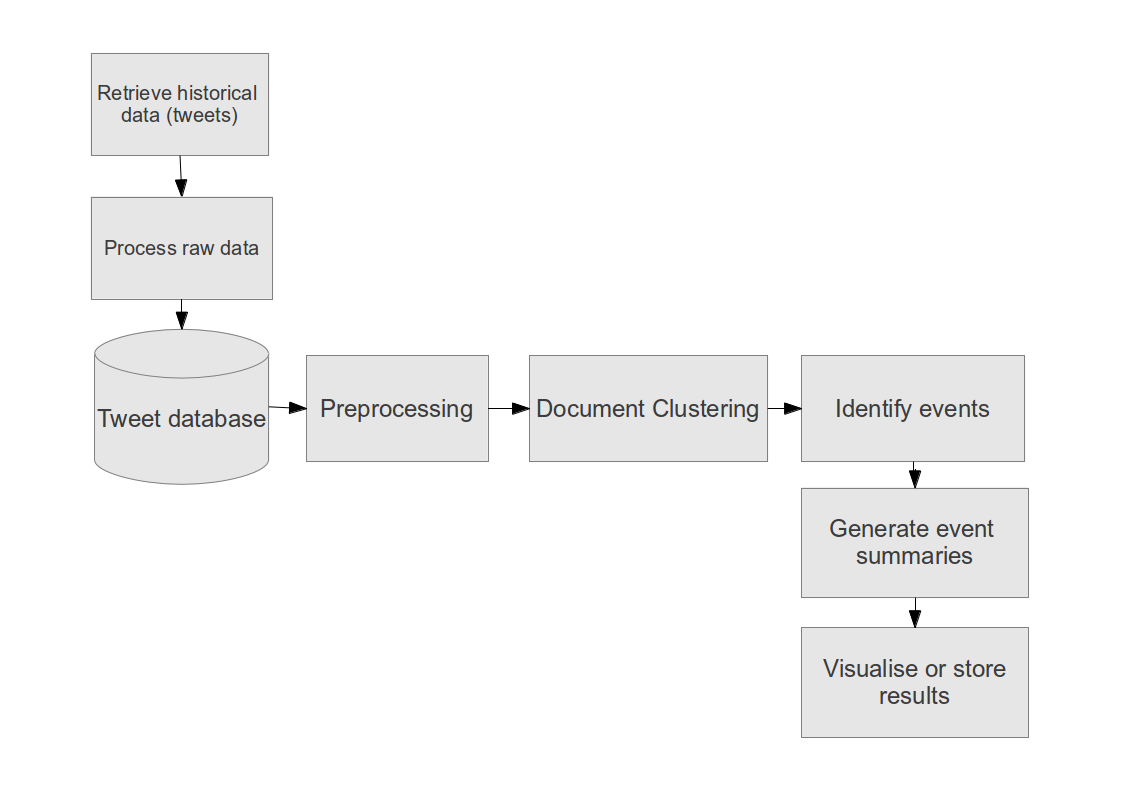
\includegraphics[height=3in, width=6in]{system-overview}
    \caption{System overview - The event extraction system comprises of several independent components.}
    \label{SystemOverview}
  \end{center}
\end{figure}

\subsection{Tools}
In the process of implementing the system we have mainly used our implementation of the algorithms but several third-party 
software libraries were used to implement the sub-components of the system. Here we describe the main tools we have used.\\ 

\begin{itemize}
 \item \textbf{Python:} 
 \item \textbf{Natural Language Toolkit (NLTK) :} 
 \item \textbf{Lucene:} 
 \item \textbf{Orange:} 
\end{itemize}\vspace{15pt}

\section{Data Retrieval}
A vital part of our system is the retrieval of a large amount of historical tweets. The first obvious choice is the Twitter API which provides tweets, user profiles and several metadata related to Twitter. They also provide a streaming API which is commonly used to collect tweets in real time. However, the main problem with the Twitter API is that it has a very restrictive limit policy (150 requests per hour) and it does not provide access to tweets posted more than a few days ago. This is a problem for our project since we require access to historical data. The solution is to use other archiving services and there are numerous possibilities. However, it is essential for us to have direct access to their database through an API and unfortunatelly, most of them do not provide an API. We have found that Topsy \footnote{http://topsy.com/} provides an excellent API \footnote{http://code.google.com/p/otterapi/} and direct access to tweets from 2009 up to the present day. Additionally, Topsy API is free and the limit policy allows us to retrieve our data easily. Therefore, we have decided to use Topsy Otter API with its Python bindings.

\section{Raw text processing}
The raw tweets received from Topsy are not processed and therefore we must apply some pre-processing steps before storing them in the database. The reasons for pre-processing were outlined clearly in Chapter \ref{TheoreticalFramework}. Figure \ref{RawTextProcessingOverview} depicts the sub-components of the raw text pre-processing module.\\

\begin{figure}[htbp]
  \begin{center}
    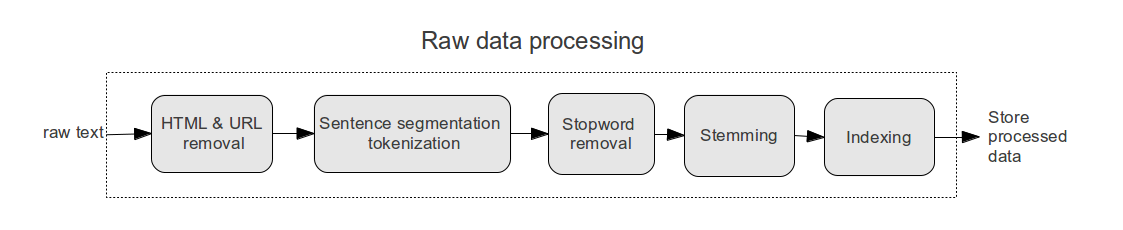
\includegraphics[height=1.5in, width=6in]{raw-data-processing}
    \caption{The raw data processing module - All the steps neccessary to convert raw documents to a format suitable for storage in a database.}
    \label{RawTextProcessingOverview}
  \end{center}
\end{figure} 

\textbf{HTML and URL removal:} Firstly, we need to clean the tweets from the URLs and HTML tags since they are useless for clustering. In order to do so we have used regular expressions which capture any possible format of URLs or HTML code.\\

\textbf{Sentence segmentation and tokenisation:} For the implementation of this module we have used the default sentence segmenter of NLTK and the WordPunctTokenizer to tokenise the resulting sentences. The reason we have used WordPunctTokenizer is due to the fact that it can handle alphabetic and non-alphabetic characters. Since it is common to use non-alphabetic characters in a tweet we could find an easy way to remove characters such as '.' and ','. Consider for example the following tweet:
 
\begin{figure}[htbp]
  \begin{center}
    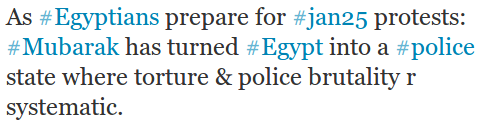
\includegraphics[height=1in, width=4in]{tweet-text}
    \label{TweetText}
  \end{center}
\end{figure}

The output from this module will be a list of words containing the terms \textbf{[ 'as', 'egyptians', 'prepare', 'for' 'jan25', 'protests', 'mumbarak', 'has', 'turned', 'egypt', 'into', 'a', 'police', 'state', 'where', 'torture', 'police', 'brutality', 'r', 'systematic' ]}. Note that characters '.', '\#', '\&' and ':' have been removed. \\

\textbf{Stopword removal:} The next step is to remove common English words that doesn't provide any information. NLTK provides a dictionary of the English stopwords and we have used it to filter out stopwords from the tweets. Using the list of words extracted for the example above the output of the stopword removal module will be: \textbf{['egyptians', 'prepare', 'jan25', 'protests', 'mumbarak', 'turned', 'egypt', 'police', 'state', 'torture', 'police', 'brutality', 'r', 'systematic' ]}

\textbf{Stemming:} Once we have the list of our terms we can use a stemming algorithm to reduce the words to their root. Our implementation uses the widely used Porter stemmer which is also implemented in NLTK. The final list of words after the stemming becomes \textbf{['egyptian', 'prepar', 'jan25', 'protest', 'mumbarak', 'turn', 'egypt', 'polic', 'state', 'tortur', 'polic', 'brutal', 'r', 'systemat' ]}\\

\textbf{Indexing:} Just before storing the tweets in the database we take a last step which is to index the tweets. For each word occuring in our corpus we aggregate all the tweets that contain that term and the position of that word in the document. Effectively, we create a mapping from a word to a list of documents. In our implementation the inverted index is very important since it allows us to construct term-documment vectors easily and filter terms and documents. For example, using our index we can find the words that appear either too often or less frequently and filter them out. This is used to reduce the dimensionality of our dataset by removing unneccesary words. Alternatively, we
can remove documents/tweets which contain keywords that appear too often or less frequently. In our implementation we have used PyLucene which is the Python equivalent of the Lucene indexing library. The library allow us to do what we have discussed above and in addition it provides helper functions such as the calculation of the TF-IDF weigtings for a dataset.
 
\section{Clustering}

\begin{lstlisting}[language=Python, label=AbstractClustererSnippet, caption=AbstractClusterer]
for word in words:
  print word
\end{lstlisting}

\section{Identifying events}

\section{Generating automatic summaries}

\section{Classifying users}

\section{Optimisations}

\section{Developing a proof-of-concept web application}\label{WebApp}

\section{Summary}

% ------------------------------------------------------------------------


%%% Local Variables: 
%%% mode: latex
%%% TeX-master: "../thesis"
%%% End: 
